\documentclass[10pt, a4paper]{article}
% \usepackage[english]{babel}
\usepackage[portuguese]{babel}
\usepackage[utf8]{inputenc}
% \usepackage[T1]{fontenc}

% matlab code
\usepackage{matlab-prettifier}
% \usepackage[numbered,framed]{matlab-prettifier}
\let\ph\mlplaceholder % shorter macro
\definecolor{codegreen}{rgb}{0,0.6,0}
\definecolor{codegray}{rgb}{0.5,0.5,0.5}
\definecolor{codepurple}{rgb}{0.58,0,0.82}
\definecolor{backcolour}{rgb}{0.95,0.95,0.92}
\lstdefinestyle{myStyle}{
%     belowcaptionskip=1\baselineskip,
    language=Matlab,
    breaklines=true,
    frame=single,
    numbers=none,
    basicstyle=\tiny,%\footnotesize\ttfamily,
    keywordstyle=\bfseries\color{magenta},
    commentstyle=\color{codegreen},
    identifierstyle=\color{blue},
    backgroundcolor=\color{backcolour},
    stringstyle=\color{codepurple},
}
\usepackage{adjustbox}

% For subfigure use
\usepackage[font=small,labelfont=bf]{caption}
\usepackage{subcaption}

% Set page size and margins
% Replace `letterpaper' with`a4paper' for UK/EU standard size
\usepackage[a4paper,top=2cm,bottom=2cm,left=2cm,right=2cm,marginparwidth=2cm]{geometry}

% tabelas
\usepackage{array}
\usepackage{tabularx}
\usepackage{booktabs}

\usepackage{float}

% Useful packages
\usepackage{amsmath}
\usepackage{undertilde}
\usepackage{graphicx}
\graphicspath{{figures/}} %Setting the graphicspath
\usepackage[colorlinks=true, allcolors=blue]{hyperref}

\title{PUC-RJ Pontif\'icia Universidade Cat\'olica do Rio de Janeiro \\ MEC 2403 - Otimiza\c c\~ao e Algoritmos para Engenhria Mec\^anica \\ Trabalho 01 - Otimiza\c c\~ao  sem Restri\c c\~oes  \\
\large Professor: Ivan Menezes}

\author{Felipe da Costa Pereira - mat. 2212376 \\ {\tt felipecostapereira@gmail.com}}
\begin{document}

\maketitle

\section{Introdu\c c\~ao}

Otimiza\c c\~ao sem restri\c c\~ao (OSR) consiste em encontrar o m\'inimo de uma fun\c c\~ao $f(\vec{x})$ onde n\~ao h\'a restri\c c\~ao em rela\c c\~ao ao dom\'inio das vari\'aveis $\vec{x}$. A fim de se encontar o minimo da fun\c c\~ao $f(\vec{x})$ a partir de um ponto de partida $(\vec{x_{0}})$ , os m\'etodos apresentados nesse trabalho consistem na repeti\c c\~ao de duas etapas principais at\'e que um crit\'erio de parada seja atingido:
\begin{enumerate}
      \item Selecionar uma dire\c c\~ao $\vec{d}$ a partir do ponto $\vec{x_{0}}$
      \item Encontrar o m\'inimo da fun\c c\~ao $f$ nessa dire\c c\~ao, chegando a um novo ponto $\vec{x_{1}} = \vec{x_{0}} + \alpha\vec{d}$, onde $\alpha$ \'e um n\'umero real.
      \item Tomar $\vec{x_{1}}$ como o novo ponto de partida $\vec{x_{0}}$
      \item Repetir os passos de 1 a 3 at\'e que uma condi\c c\~ao de parada seja atingida: m\'inimo encontrado ($|\vec{\nabla f}|=0$), ou m\'aximo n\'umero de itera\c c\~oes atingido.
\end{enumerate}

Dessa forma o problema de minimiza\c c\~ao da fun\c c\~ao $f(\vec{x})$ se torna um problema de sucessivas determina\c c\~oes de dire\c c\~oes de busca e suas respectivas buscas lineares nesssas dire\c c\~oes.

\section{Objetivos}

Os principais objetivos deste trabalho s\~ao:
\begin{itemize}
      \item Implementar numericamente os algoritmos de otimiza\c c\~ao: Univariante, Powell, Steepest Descent, Fletcher-Reeves, Newton-Raphson e BFGS.
      \item Avaliar a influ\^encia dos par\^ametros dos algoritmos nas m\'etricas de converg\^encia e comparar essas \'ulltimas com os valores esperados da teoria.
      \item Aplicar os algoritmos implementados na solu\c c\~ao do problema de OSR em tr\^es casos: uma fun\c c\~ao quadr\'atica, uma n\~ao quadr\'atica e uma terceira fun\c c\~ao que representa um problema de engenharia (minimizaz\c c\~ao da energia de um sistema massa-mola visando encontrar seu ponto de equil\'ibrio est\'atico)
\end{itemize}

\section{Algoritmos de Busca Linear}
\subsection{Passo Constante}
\subsection{Bisse\c c\~ao}
\subsection{Se\c c\~ao \'Aurea}
\section{Algoritmos de dire\c c\~ao}
\subsection{Univariante}
\subsection{Powell}
\subsection{Steepest Descent}
\subsection{Fletcher-Reeves}
\subsection{Newton-Raphson}
\subsection{BFGS}

\section{Metodologia}

Para atingir os objetivos do trabalho, foram programados scripts em linguagem Matlab, organizados conforme esquematizado na figura \ref{fig:fluxo}.

\begin{figure}[H]
      \centering
      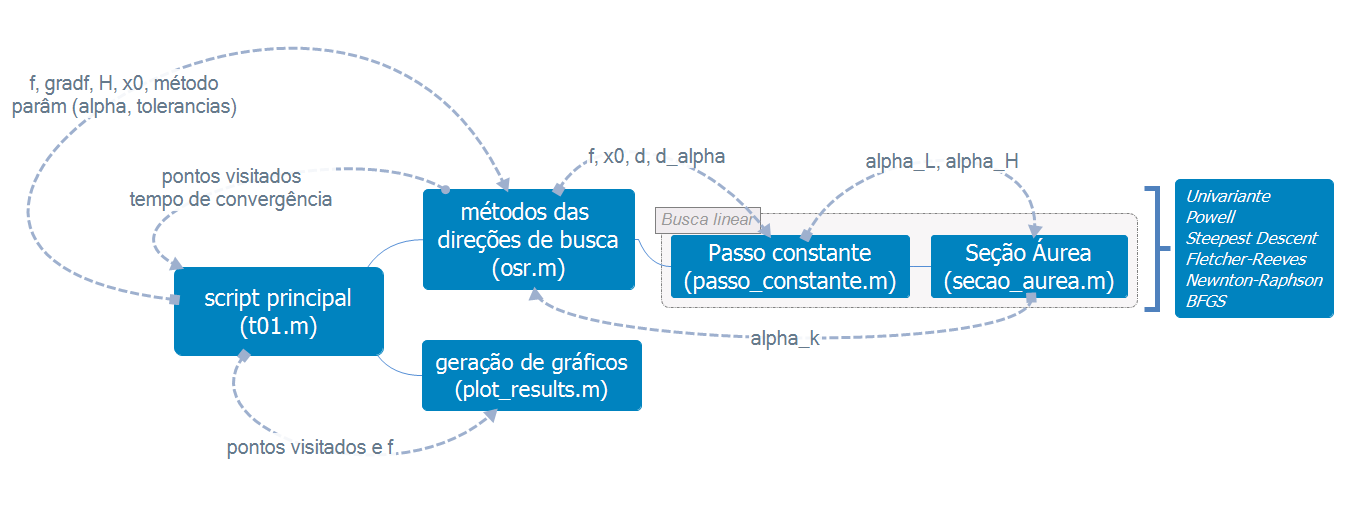
\includegraphics[width=.9\textwidth]{t01.png}
      \caption{Fluxo dos scripts}
      \label{fig:fluxo}
\end{figure}

Um script principal \textit{t01.m} escolhe os par\^ametros do algoritmo: $\alpha$ da busca linear, m\'aximo n\'umero de itera\c c\~oes e toler\^ancias para avaliar a converg\^encia. Al\'em disso esse script cria as fun\c c\~oes, seus gradientes, matriz Hessiana e pontos iniciais, a serem passados como par\^ametros para o script que implementa os algoritmos, conforme ilustrado na listagem \ref{l1}

\begin{minipage}{\linewidth}
      \begin{lstlisting}[style=myStyle, caption=script t01.m setando par\^ametros e criando as fun\c c\~oes, label=l1]
            % dados do item 01a, f, grad f, hess f e x0
            fa = @(x) x(1)^2-3*x(1)*x(2)+4*x(2)^2+x(1)-x(2);
            gfa = @(x) [2*x(1)-3*x(2)+1 ; -3*x(1)+8*x(2)-1];
            Ha = @(x) [2 -3;-3 8];
            x01 = [2;2];
            x02 = [-1;-3];

            % parametros dos algoritmos
            iter_max = 100;
            a = 0.002; % passo
            TOL = 1e-4; % parada do gradiente
            TOL2 = 1e-7; % busca linear

            methods = ["Univariante","Powell","Steepest Descent","Fletcher Reeves","Newton-Raphson","BFGS"];
      \end{lstlisting}
\end{minipage} \\

Em seguida, o script \textit{t01.m} chama o script \textit{osr.m} para cada m\'etodo e plota as curvas de n\'ivel da fun\c c\~ao f e todos os pontos visitados durante a busca do algoritmo, atrav\'es do script \textit{plot\_result.m} (listagem \ref{l2})

\begin{minipage}{\linewidth}
      \begin{lstlisting}[style=myStyle, caption=script t01.m chamando o script osr.m para a fun\c c\~ao do item 1a para cada um dos 6 m\'etodos estudados., , label=l2]
            fprintf('\n******************** ITEM 01A ************************\n');
            for method = 1:6
                fprintf('---%s---\n', methods(method));

                fprintf('x0=[%2d,%2d]: ',x01(1), x01(2));
                [x_1,t] = osr (fa, gfa, Ha, x01, method, iter_max, a, TOL, TOL2);
                fprintf('(%.1fms), xmin=[%0.4f,%0.4f], f=%0.4f\n', t*1000, x_1(1,end), x_1(2,end), fa(x_1(:,end)));

                fprintf('x0=[%2d,%2d]: ',x02(1), x02(2));
                [x_2,t] = osr (fa, gfa, Ha, x02, method, iter_max, a, TOL, TOL2);
                fprintf('(%.1fms), xmin=[%0.4f,%0.4f], f=%0.4f\n', t*1000, x_2(1,end), x_2(2,end), fa(x_2(:,end)));

                plot_result(min([x_1(1,:), x_2(1,:)])-dx,max([x_1(1,:), x_2(1,:)])+dx,min([x_1(2,:), x_2(2,:)])-dx,max([x_1(2,:), x_2(2,:)])+dx, x_1, x_2, methods(method), 1)
                exportgraphics(gcf,strcat('./figures/img01A_m0',num2str(method),'.png'),'Resolution',500)
            end
      \end{lstlisting}
\end{minipage} \\

O script \textit{osr.m} implementa de fato os algoritmos, recebe, retorna

\begin{minipage}{\linewidth}
      \begin{lstlisting}[style=myStyle, caption=script osr.m implementando o m\'etodo de Powell, label=list_osr]
            function [x_,time_elap] = osr (f, gf, H, x0, method, iter_max, a, TOL, TOL2)
            % 1. Univariante
            % 2. Powell
            % 3. Steepest Descent
            % 4. Flecher?Reeves
            % 5. Newton?Raphson
            % 6. BFGS

            k=0;
            conv=0; %flag convergencia
            tstart = tic;
            switch method
                case 2
                % 2. Powell
                    x_ = x0;
                    x = x0;
                    while k < iter_max
                        j = 1;
                        n = 2;
                        y = [[1;0],[0;1]];
                        while j <= n
                            [alpha_L, alpha_H] = passo_constante(f, x, y(:,1), a);
                            alpha_k = secao_aurea(f, x, y(:,1), TOL2, alpha_L, alpha_H);
                            k=k+1;
                            x = x + alpha_k*y(:,1);
                            x_ = [x_,x];
                            [alpha_L, alpha_H] = passo_constante(f, x, y(:,2), a);
                            alpha_k = secao_aurea(f, x, y(:,2), TOL2, alpha_L, alpha_H);
                            k=k+1;
                            x = x + alpha_k*y(:,2);
                            x_ = [x_,x];
                            d = x-x0;
                            [alpha_L, alpha_H] = passo_constante(f, x, d, a);
                            alpha_k = secao_aurea(f, x, d, TOL2, alpha_L, alpha_H);
                            k=k+1;
                            x0 = x + alpha_k*d;
                            x=x0;
                            x_ = [x_,x];

                            y(:,1) = y(:,2);
                            y(:,2) = d;

                            j = j+1;
                        end
                        if norm(gf(x)) < TOL
                            fprintf('%d steps!', k);
                            conv=1;
                            break;
                        end
                    end
                    if conv == 0
                        fprintf('Nao convergiu apos %d steps', k);
                    end
      \end{lstlisting}
\end{minipage}






\section{Resultados}

\section{Conclu\~oes}

In order to use the Tustin model for the friction force as proposed, the torque expression changes from equation \ref{eq:1} to equation \ref{eq:2} described below:     \newline


Torque expression using Coulomb friction force model:
\begin{equation}\label{eq:1}
      \tau(t) = M\ddot{q}(t) + F_{v}\dot{q}(t) + F_{c}sign(\dot{q}(t)) + offset
\end{equation}

Torque expression using Tustin friction force model:
\begin{equation}\label{eq:2}
      \tau(t) = M\ddot{q}(t) + F_{v}\dot{q}(t) + F_{c}sign(\dot{q}(t)) + (F_{s} - F_{c})e^{-\frac{|\dot{q}|}{v_{s}}} + offset
\end{equation}


Parameters and $\dot{x_{2}}=\ddot{q}$ expresion on the state vector: \\

\definecolor{codegreen}{rgb}{0,0.6,0}
\definecolor{codegray}{rgb}{0.5,0.5,0.5}
\definecolor{codepurple}{rgb}{0.58,0,0.82}
\definecolor{backcolour}{rgb}{0.95,0.95,0.92}

The range for the $v_{s}$ parameter was based on the respecitve value given by the IDIM model ($v_{s} = 0.006464$). The rest of the code is kept exactly the same.

\section{Results}

After performing the grey box identification using the casadi library, we compare the parameters values estimated by the inverse dynamic model (IDM) and the grey box casadi model. The values of the estiamted parameters, for both the Coulomb and the Tustin friction forces are shown in tables \ref{table:m1} and \ref{table:m2}.

\begin{table}[H]
      \small
      \centering
      \caption{Coulomb Model parameters}
      \begin{tabular}{c|c|c|c|c}
            Model &  M & Fv & Fc & ofst \\
            \hline
            casadi & 95.1089 & 203.5034 & 20.3935 & -3.1648 \\
            IDIM   & 96.0014 & 213.8943 & 19.4167 & -3.2790 \\
      \end{tabular}
      \label{table:m1}
\end{table}

\begin{table}[H]
      \small
      \centering
      \caption{Tustin Model parameters}
      \begin{tabular}{c|c|c|c|c|c|c}
            Model &  M & Fv & Fc & Fs & vs & ofst \\
            \hline
            casadi & 97.001 & 222.01 & 18.606 & 36.3311 & 0.000900 & -3.29 \\
            IDIM   & 95.681 & 203.36 & 17.023 & 17.0230 & 0.006464 & -4.12 \\
      \end{tabular}
      \label{table:m2}
\end{table}

The simulated responses and the associeted errors, for both force models (Coulomb and Tustin) and parameters estimation methods (casadi amd IDIM) are show in figures \ref{fig:y} and \ref{fig:e}.

As we can notice, casadi models estimate have a good fit for both force models, while IDIM models have a poor performace (higher error) when estimating the Tustin force model parameters.

\begin{figure}[H]
      \centering
      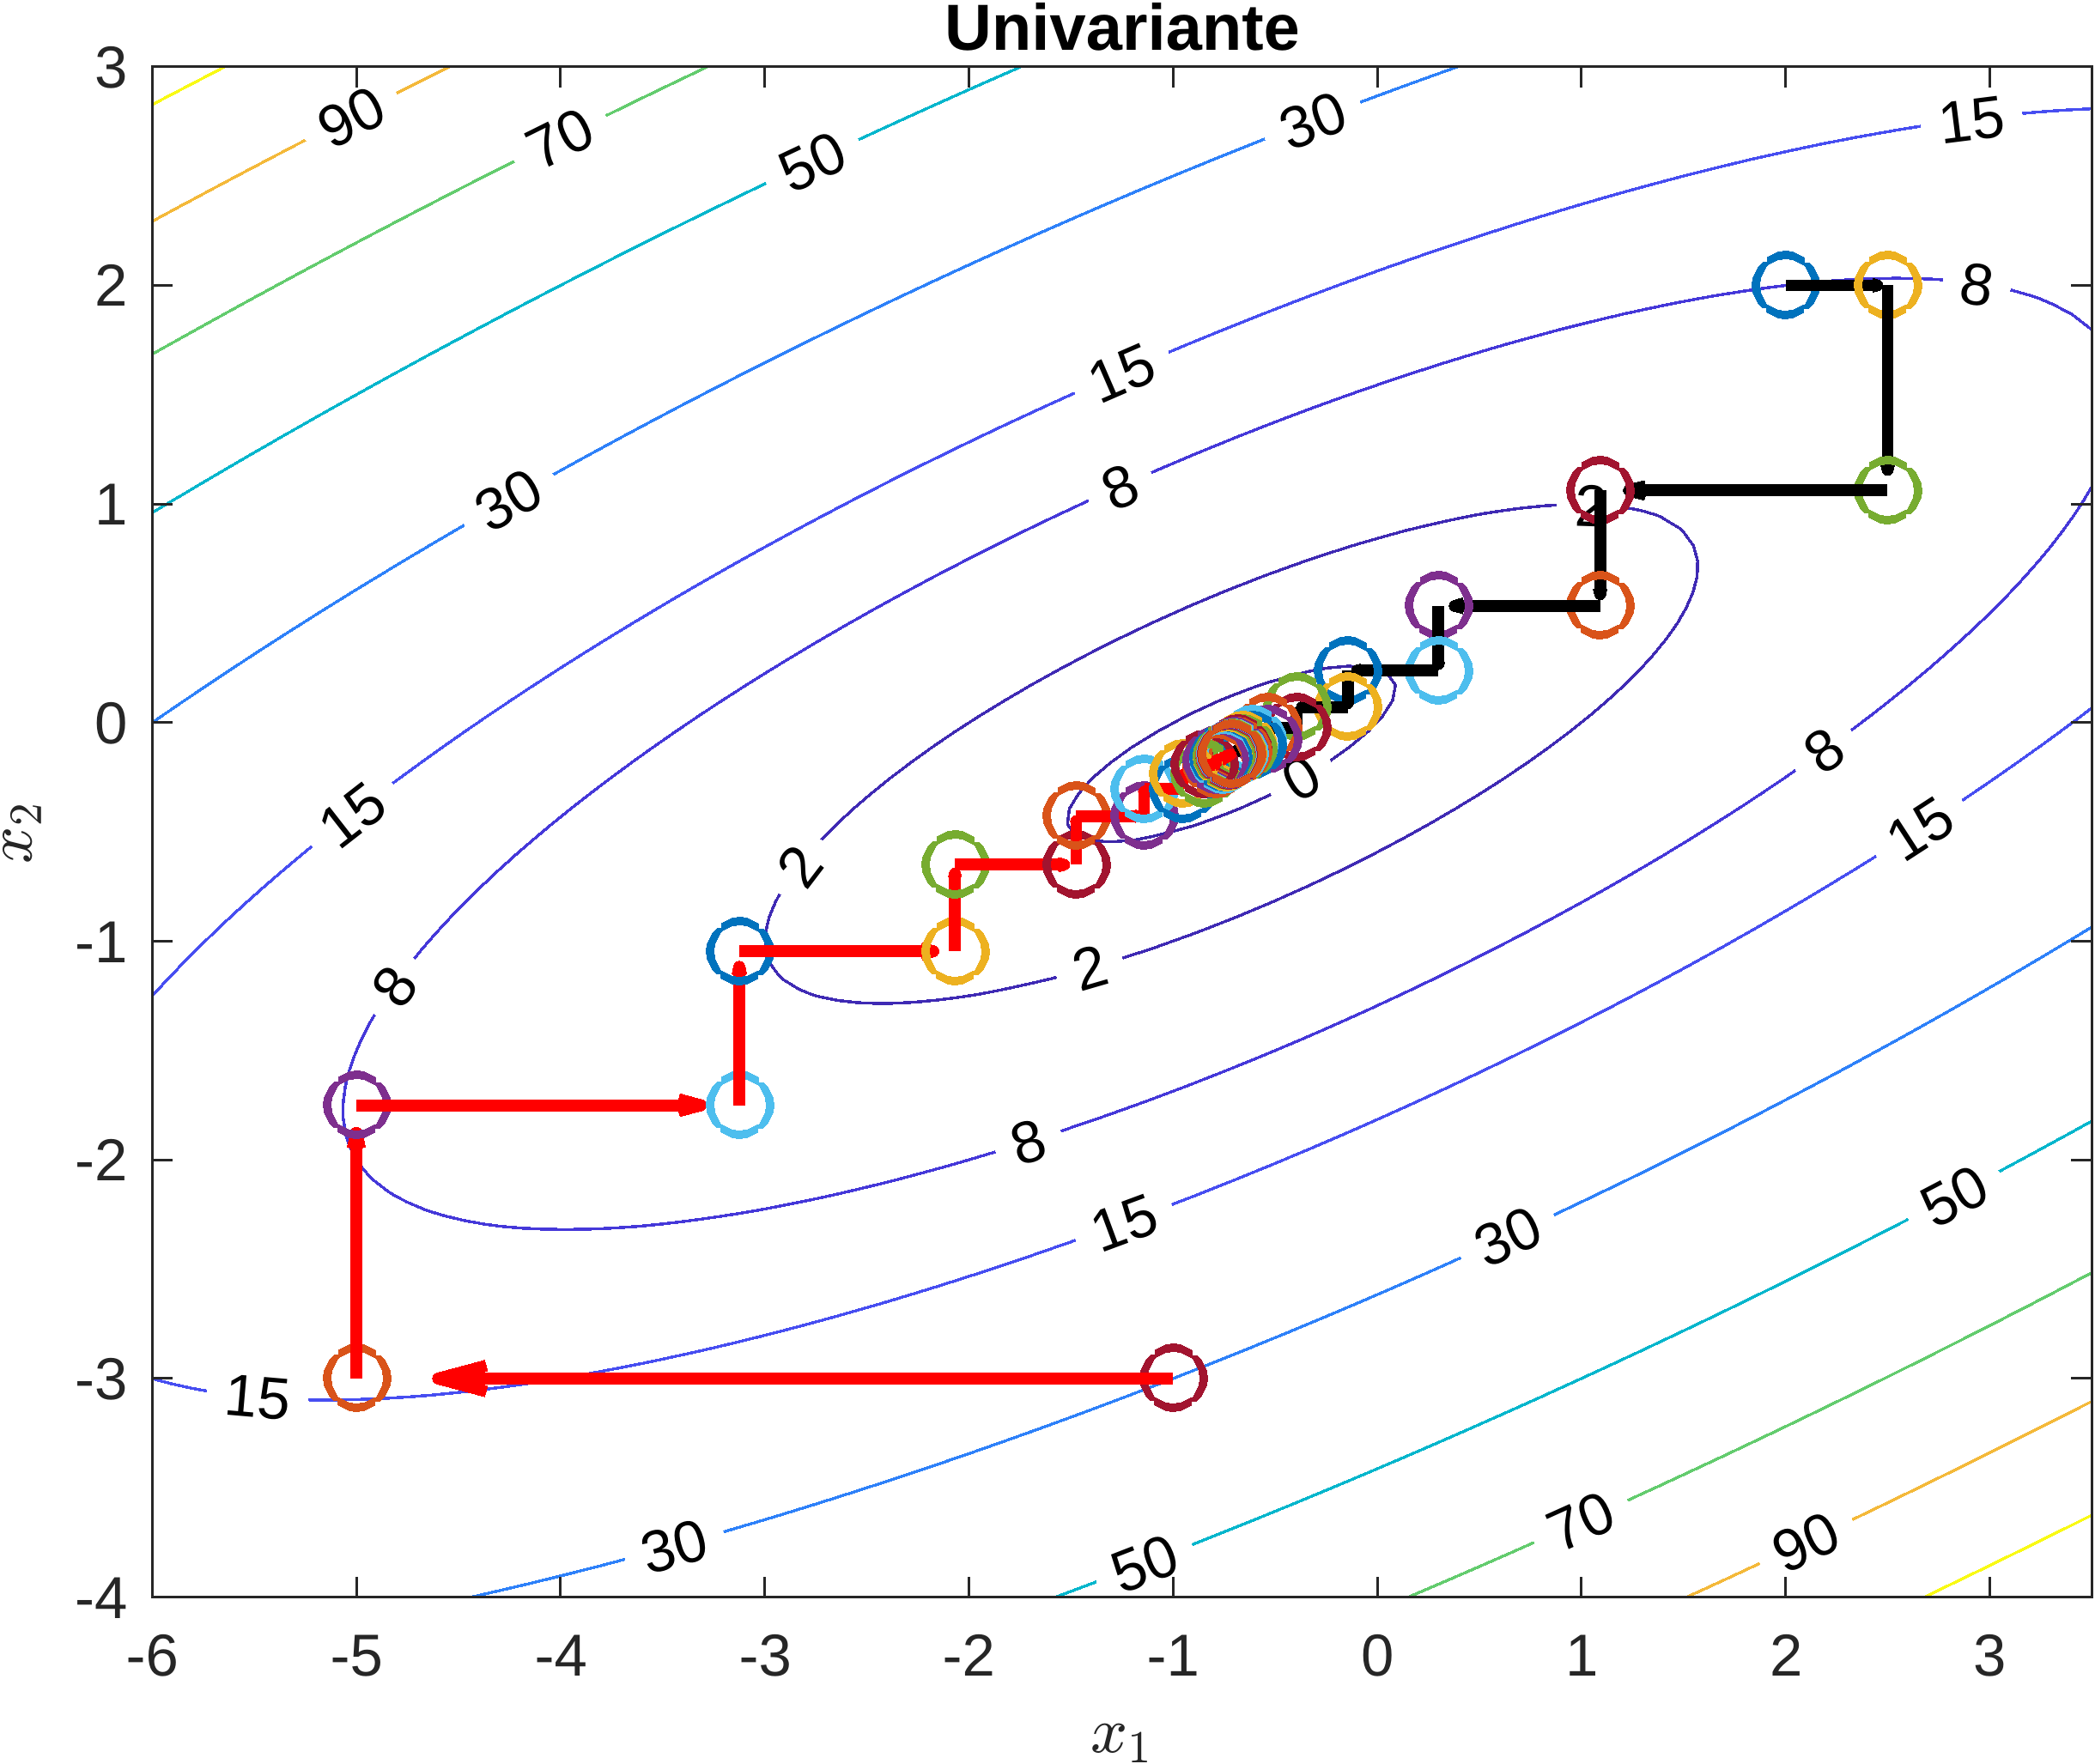
\includegraphics[width=\textwidth]{img01A_m01.png}
      \caption{Position (y) - real and estimated dsata}
      \label{fig:y}
\end{figure}

\begin{figure}[H]
      \centering
      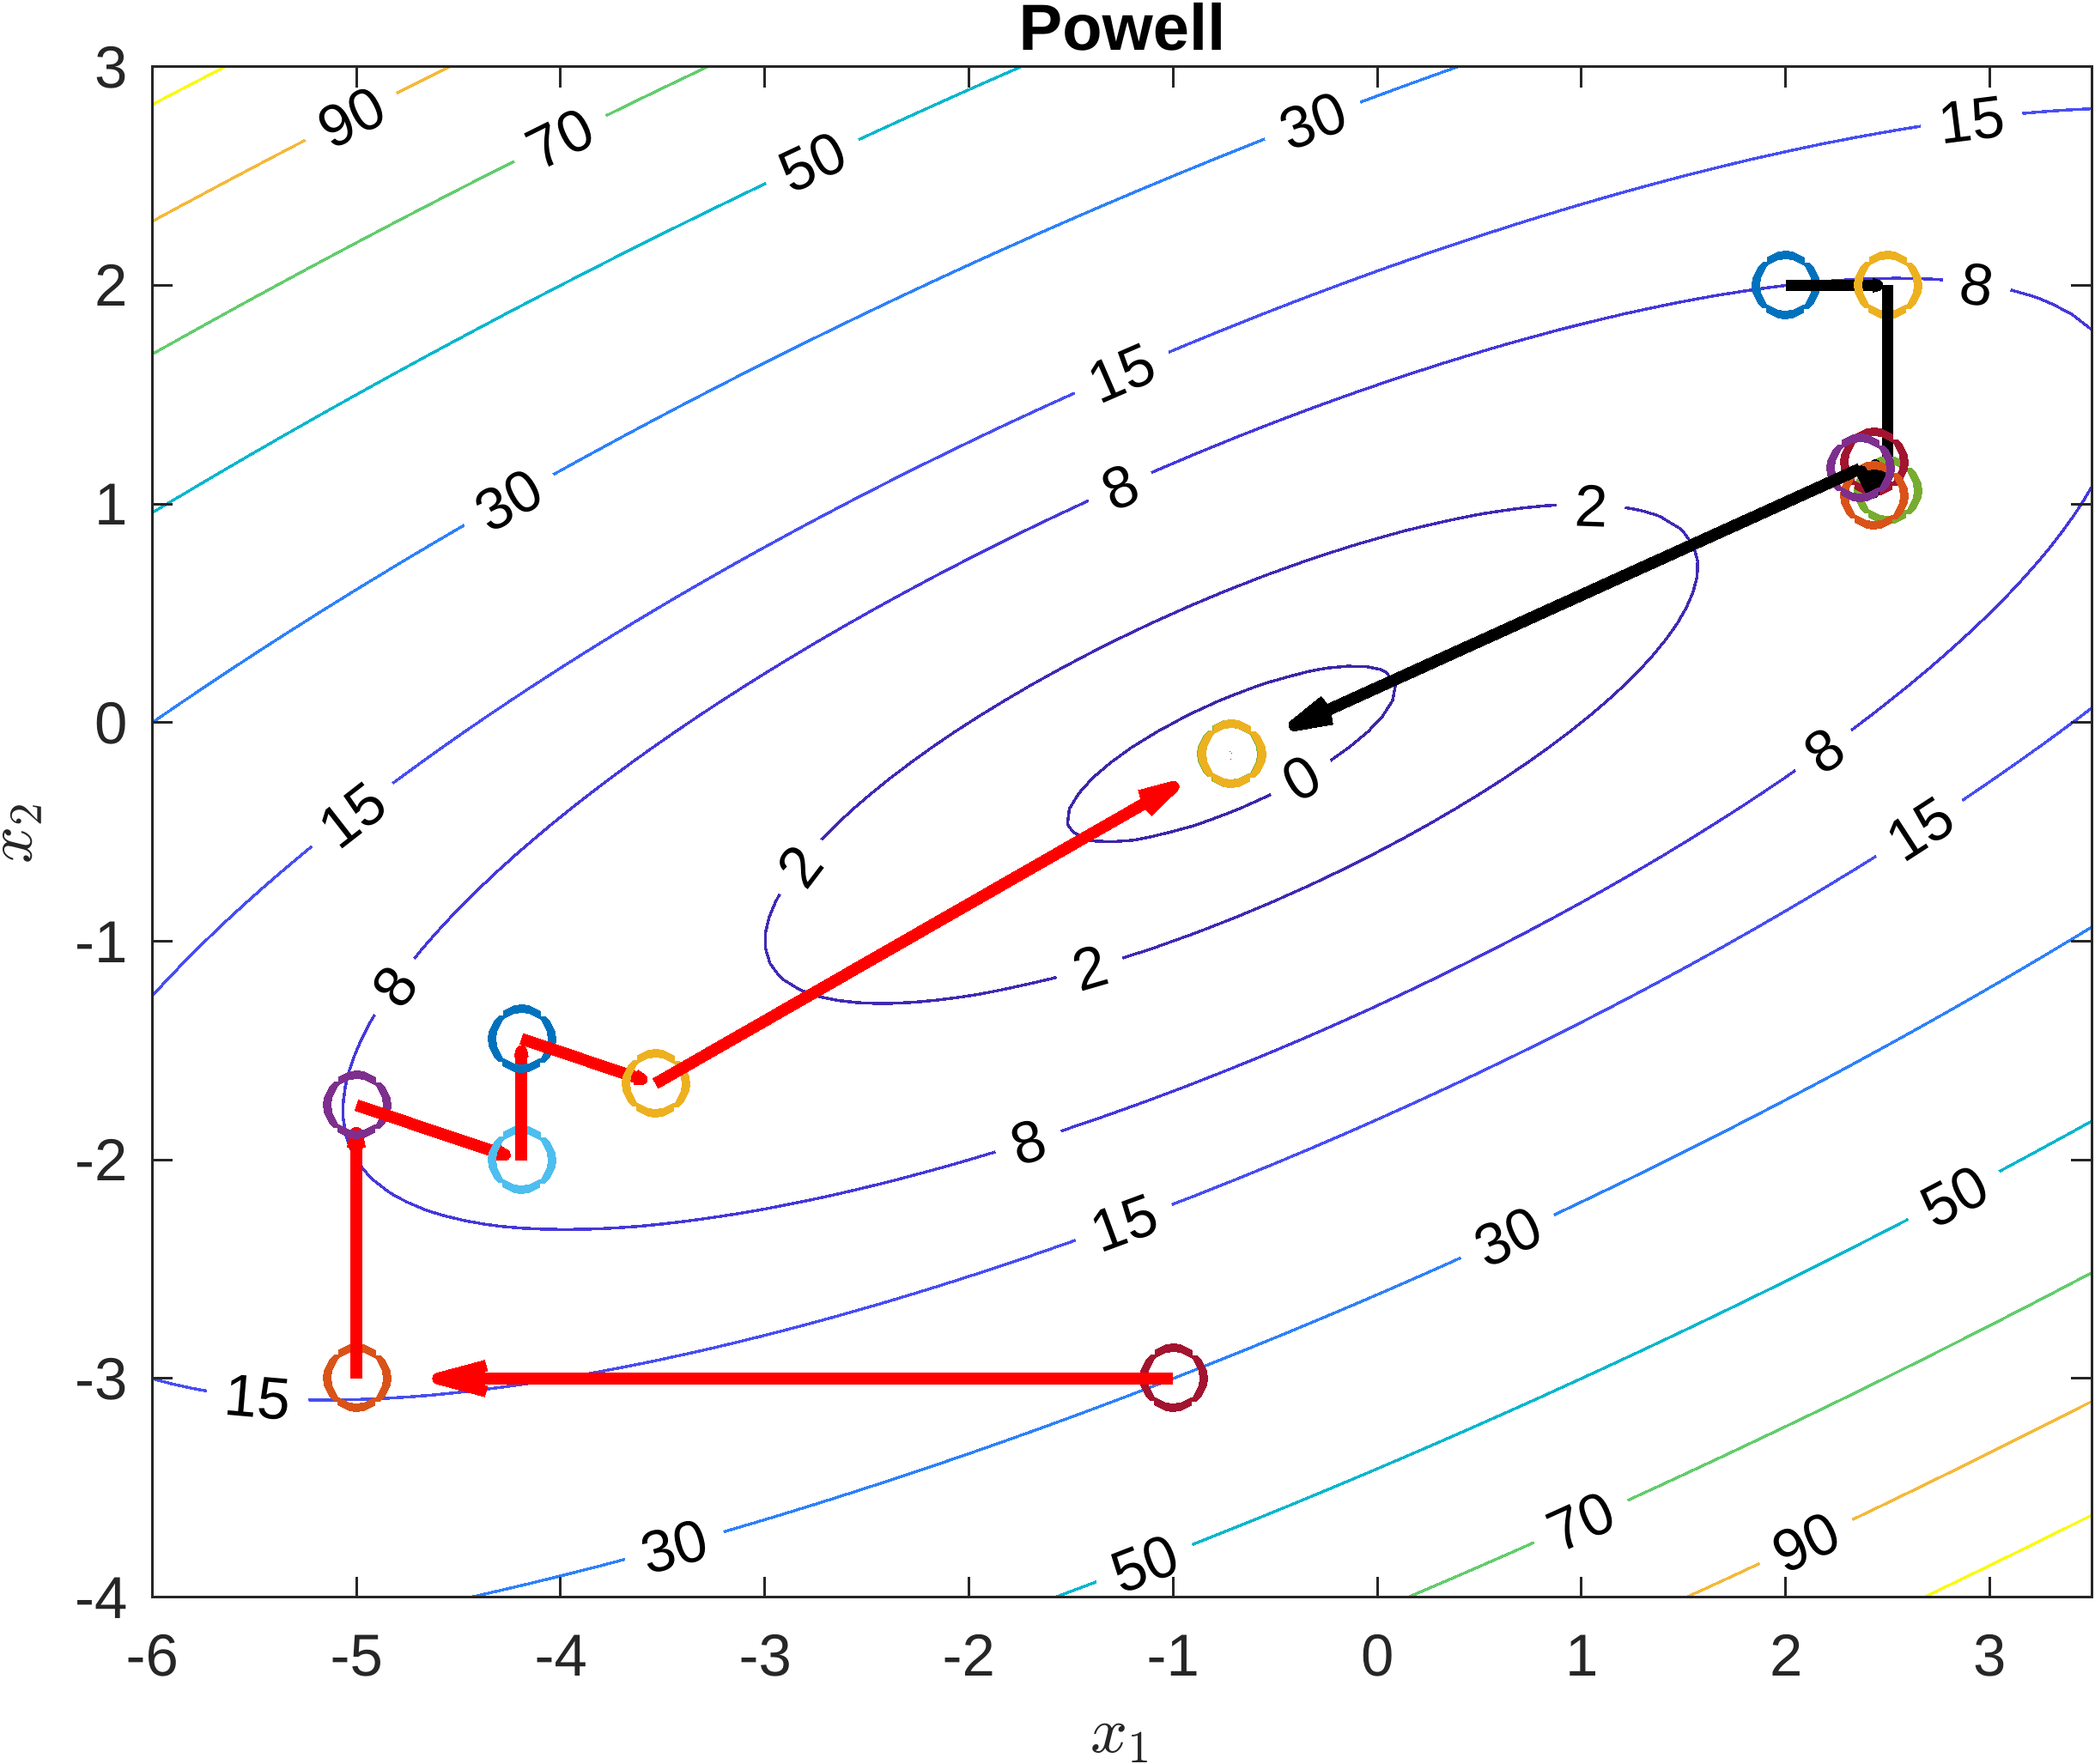
\includegraphics[width=\textwidth]{img01A_m02.png}
      \caption{Error between estimated and real data}
      \label{fig:e}
\end{figure}

\end{document}
